%************************************************
\chapter[Appendix 3.2: Chapter 3 - Supplementary results]{Appendix 3.2: Chapter 3 - Supplementary results}\label{ch:Appendix3.2}
%************************************************
\renewcommand{\thefigure}{A.3.2.\arabic{figure}}
\setcounter{figure}{0}

\renewcommand{\thetable}{A.3.2.\arabic{table}}
\setcounter{table}{0}

Here we present the results of the statistical tests associated with \cref{fig:fig3.2},\cref{fig:fig3.3}, and \cref{fig:fig3.4} of Chapter 3. In addition, we show how persistence values, i.e. \cref{fig:fig3.2} of Chapter 3, vary across trophic levels (Fig. \ref{fig:figApp3.2.1}), and how average species impact vary with increasing species richness \ref{fig:figApp3.2.1}). In the following tables, the following abbreviations are used referring to simulations with varying interaction frequencies: ER = Equal ratio among interaction types, HAM = High amensalism, HAN = High antagonism, HCM = High commensalism, HCP = High competition, HM = High mutualism.

\subsection*{1. Differences between persistence levels across simulations (Fig. \cref{fig:fig3.2} of Chapter 3)}\label{persistence-differences}

We tested whether the distributions of persistence values for each category of interaction frequency were different or not. For that, we grouped the observations according to the initial richness of the simulations and, for each level of initial richness, we performed a Kruskal-Wallis rank test for differences in the distributions of persistence across the six levels of interaction frequencies (Table \ref{tab:tableApp3.2.1}). Kruskal-Wallis test are non-parametric tests appropriate for testing whether sets of samples originate from the same distribution. These tests showed significant differences between persistence distributions within each richness level, so we performed post-hoc Dunn tests for the difference between every pair of distributions, again within each richness level (Table \ref{tab:tableApp3.2.2}). P-values were adjusted with the Bonferroni correction. All pairs of distributions were significantly different except that of the ``equal ratio'' and ``high antagonism'' simulations with 40 initial species.

\begin{longtable}[]{@{}lrrr@{}}
\caption[Kruskal-Wallis tests for persistence distributions]{\color{Gray}Kruskal-Wallis rank tests for differences between pairs of persistence distributions.}\label{tab:tableApp3.2.1}\\
\toprule
Initial richness & \(\chi^2\) & Df & p-value\tabularnewline
\midrule
\endhead
20 & 1430.6 & 5 & \textless{} 0.001\tabularnewline
40 & 1349.6 & 5 & \textless{} 0.001\tabularnewline
60 & 552.69 & 5 & \textless{} 0.001\tabularnewline
\bottomrule
\end{longtable}

\begin{longtable}[]{@{}llll@{}}
\caption[Post-hoc Dunn tests for persistence distributions]{\color{Gray}Pair-wise post-hoc Dunn's test comparisons for every pair of simulations.}\label{tab:tableApp3.2.2}\\
\toprule
Pair & Initial richness & Z statistic & p-value\tabularnewline
\midrule
\endfirsthead
\toprule
Pair & Initial richness & Z statistic & p-value\tabularnewline
\midrule
\endhead

ER - HAM & 20 & 7.657 & \textless{} 0.001\tabularnewline
ER - HAM & 40 & 8.388 & \textless{} 0.001\tabularnewline
ER - HAM & 60 & 8.589 & \textless{} 0.001\tabularnewline
ER - HAN & 20 & 3.909 & \textless{} 0.001\tabularnewline
ER - HAN & 40 & 0.559 & 1\tabularnewline
ER - HAN & 60 & 4.019 & \textless{} 0.001\tabularnewline
ER - HCM & 20 & -7.388 & \textless{} 0.001\tabularnewline
ER - HCM & 40 & -8.674 & \textless{} 0.001\tabularnewline
ER - HCM & 60 & -3.971 & \textless{} 0.001\tabularnewline
ER - HCP & 20 & 13.56 & \textless{} 0.001\tabularnewline
ER - HCP & 40 & 12.89 & \textless{} 0.001\tabularnewline
ER - HCP & 60 & 12.04 & \textless{} 0.001\tabularnewline
ER - HM & 20 & -20.09 & \textless{} 0.001\tabularnewline
ER - HM & 40 & -19.21 & \textless{} 0.001\tabularnewline
ER - HM & 60 & -7.414 & \textless{} 0.001\tabularnewline
HAM - HAN & 20 & -3.749 & 0.0013\tabularnewline
HAM - HAN & 40 & -7.829 & \textless{} 0.001\tabularnewline
HAM - HAN & 60 & -4.569 & \textless{} 0.001\tabularnewline
HAM - HCM & 20 & -15.045 & \textless{} 0.001\tabularnewline
HAM - HCM & 40 & -17.062 & \textless{} 0.001\tabularnewline
HAM - HCM & 60 & -12.56 & \textless{} 0.001\tabularnewline
HAM - HCP & 20 & 5.903 & \textless{} 0.001\tabularnewline
HAM - HCP & 40 & 4.497 & \textless{} 0.001\tabularnewline
HAM - HCP & 60 & 3.452 & 0.0042\tabularnewline
HAM - HM & 20 & -27.75 & \textless{} 0.001\tabularnewline
HAM - HM & 40 & -27.59 & \textless{} 0.001\tabularnewline
HAM - HM & 60 & -16.004 & \textless{} 0.001\tabularnewline
HAN - HCM & 20 & -11.297 & \textless{} 0.001\tabularnewline
HAN - HCM & 40 & -9.233 & \textless{} 0.001\tabularnewline
HAN - HCM & 60 & -7.991 & \textless{} 0.001\tabularnewline
HAN - HCP & 20 & 9.651 & \textless{} 0.001\tabularnewline
HAN - HCP & 40 & 12.33 & \textless{} 0.001\tabularnewline
HAN - HCP & 60 & 8.021 & \textless{} 0.001\tabularnewline
HAN - HM & 20 & -24.01 & \textless{} 0.001\tabularnewline
HAN - HM & 40 & -19.77 & \textless{} 0.001\tabularnewline
HAN - HM & 60 & -11.43 & \textless{} 0.001\tabularnewline
HCM - HCP & 20 & 20.95 & \textless{} 0.001\tabularnewline
HCM - HCP & 40 & 24.56 & \textless{} 0.001\tabularnewline
HCM - HCP & 60 & 16.01 & \textless{} 0.001\tabularnewline
HCM - HM & 20 & -12.71 & \textless{} 0.001\tabularnewline
HCM - HM & 40 & -10.53 & \textless{} 0.001\tabularnewline
HCM - HM & 60 & -3.44 & 0.0043\tabularnewline
HCP - HM & 20 & -33.66 & \textless{} 0.001\tabularnewline
HCP - HM & 40 & -32.09 & \textless{} 0.001\tabularnewline
HCP - HM & 60 & -19.46 & \textless{} 0.001\tabularnewline
\bottomrule

\end{longtable}

\subsection*{2. Differences between the initial and final frequencies of interaction (\cref{fig:fig3.3} of Chapter 3)}\label{Interaction-frequencies}

For testing the difference between the initial and final frequency of each interaction type, we performed Wilcoxon paired signed-rank tests for each combination of initial richness and level of interaction frequency. These tests allow a non-parametric analysis of the difference between paired samples. In our case, each paired sample was the initial and final frequency of a given interaction type. In particular, for each replicate of each simulation, we calculated whether the mean rank of the initial-final differences was either less, different or greater than zero. These alternative hypotheses were selected based on a preliminary inspection of the data.

\begin{longtable}[]{@{}lllll@{}}
\caption[Distribution of interaction frequencies]{\color{Gray}Wilcoxon paired signed-rank tests for testing differences between the initial and final frequency of each interaction type (\cref{fig:fig3.3}). The interaction type column refers to the set of interactions analysed. For example, ``amensalism'' refers to the ratio of amensalistic interactions in all simulations, e.g. the whole set of points from the upper-left panel, while ``amensalism - HAM'' refers to the set of amensalistic interactions in the simulation with high initial amensalism, e.g. the set of blue points in the upper-left panel. The p-values listed here correspond to the graphical legend of \cref{fig:fig3.3}.}\label{tab:tableApp3.2.3}\\

\toprule
Initial richness & Interaction type & alternative hypothesis & Statistic & P-value\tabularnewline
\midrule
\endfirsthead
\toprule
Initial richness & Interaction type & alternative hypothesis & Statistic & P-value\tabularnewline
\midrule
\endhead

20 & amensalism & initial \textgreater{} final & 10268730 & \textless{}
0.001\tabularnewline
20 & antagonism & initial \textgreater{} final & 11714319 & \textless{}
0.001\tabularnewline
20 & commensalism & initial \textless{} final & 6224456 & \textless{}
0.001\tabularnewline
20 & competition & initial \textgreater{} final & 12883361 & \textless{}
0.001\tabularnewline
20 & mutualism & initial \textless{} final & 2776289 & \textless{}
0.001\tabularnewline
20 & amensalism - HAM & initial \textgreater{} final & 270371 &
\textless{} 0.01\tabularnewline
20 & antagonism - HAN & initial \textgreater{} final & 325119 &
\textless{} 0.001\tabularnewline
20 & commensalism - HCM & initial \textless{} final & 111677 &
\textless{} 0.001\tabularnewline
20 & competition - HCP & initial \textgreater{} final & 369222 &
\textless{} 0.001\tabularnewline
20 & mutualism - HM & initial \textless{} final & 14319 & \textless{}
0.001\tabularnewline
40 & amensalism & initial \textgreater{} final & 12107905 & \textless{}
0.001\tabularnewline
40 & antagonism & initial != final & 9150881 & 0.084\tabularnewline
40 & commensalism & initial \textless{} final & 7655927 & \textless{}
0.001\tabularnewline
40 & competition & initial \textgreater{} final & 13361816 & \textless{}
0.001\tabularnewline
40 & mutualism & initial \textless{} final & 2669916 & \textless{}
0.001\tabularnewline
40 & amensalism - HAM & initial \textgreater{} final & 288792 &
\textless{} 0.001\tabularnewline
40 & antagonism - HAN & initial != final & 238615 & 0.249\tabularnewline
40 & commensalism - HCM & initial \textless{} final & 178367 &
\textless{} 0.001\tabularnewline
40 & competition - HCP & initial \textgreater{} final & 274399 &
\textless{} 0.01\tabularnewline
40 & mutualism - HM & initial \textless{} final & 2259 & \textless{}
0.001\tabularnewline
60 & amensalism & initial \textgreater{} final & 16351320 & \textless{}
0.001\tabularnewline
60 & antagonism & initial \textless{} final & 2340004 & \textless{}
0.001\tabularnewline
60 & commensalism & initial \textgreater{} final & 11596381 &
\textless{} 0.001\tabularnewline
60 & competition & initial \textgreater{} final & 16700652 & \textless{}
0.001\tabularnewline
60 & mutualism & initial \textless{} final & 579985 & \textless{}
0.001\tabularnewline
60 & amensalism - HAM & initial \textgreater{} final & 449342 &
\textless{} 0.01\tabularnewline
60 & antagonism - HAN & initial \textless{} final & 33262 & \textless{}
0.001\tabularnewline
60 & commensalism - HCM & initial \textgreater{} final & 352325 &
\textless{} 0.001\tabularnewline
60 & competition - HCP & initial \textgreater{} final & 412015 &
\textless{} 0.001\tabularnewline
60 & mutualism - HM & initial \textless{} final & 137 & \textless{}
0.001\tabularnewline
\bottomrule

\end{longtable}

\subsection*{3. Structural patterns of the model communities (\cref{fig:fig3.4} of Chapter 3)}

We checked the skewness of the distribution of species impacts by calculating the Pearson's moment coefficient of skewness for every simulation (Table \ref{tab:tableApp3.2.4}). Furthermore, we analyzed the differences between distributions of species impact per trophic level. For that, we performed a Kruskal-Wallis test followed by post-hoc Dunn tests, in a similar vein to the tests of section \textbf{1}. In this case, all pairs of species impacts distributions were significantly different.

\begin{longtable}[]{@{}lll@{}}
\caption[Skewness of species impacts]{\color{Gray} Pearson's moment coefficient of skewness of the distribution of net species impacts per simulation type (in panel a of \cref{fig:fig3.4} of Chapter 3, the simulation with 60 species and equal ratio between interactions is depicted}\label{tab:tableApp3.2.4}\\

Initial richness & Frequency of interaction types & Skewness\tabularnewline
\midrule
\endfirsthead
\toprule
Initial richness & Frequency of interaction types & Skewness\tabularnewline
\midrule
\endhead

20 & Equal ratio & 12.6\tabularnewline
20 & High amensalism & 22.1\tabularnewline
20 & High antagonism & 18.7\tabularnewline
20 & High commensalism & 7.7\tabularnewline
20 & High competition & 24.1\tabularnewline
20 & High mutualism & 8.9\tabularnewline
40 & Equal ratio & 11.2\tabularnewline
40 & High amensalism & 20.2\tabularnewline
40 & High antagonism & 20.2\tabularnewline
40 & High commensalism & 8.9\tabularnewline
40 & High competition & 19.8\tabularnewline
40 & High mutualism & 11.5\tabularnewline
60 & Equal ratio & 14.7\tabularnewline
60 & High amensalism & 20.3\tabularnewline
60 & High antagonism & 15.0\tabularnewline
60 & High commensalism & 10.3\tabularnewline
60 & High competition & 18.3\tabularnewline
60 & High mutualism & 15.0\tabularnewline
\bottomrule

\end{longtable}

\begin{longtable}[]{@{}lrlrr@{}}
\caption[Trophic-level impacts]{\color{Gray} Kruskal-Wallis rank tests for two-tail differences between average impact per trophic level (in panel b of \cref{fig:fig3.4} of Chapter 3, the simulation with 60 species and equal ratio between interactions is depicted)}\label{tab:tableApp3.2.5}\\

\toprule
Initial richness & Frequency of interaction type & s \(\chi^2\) & Df & p-value\tabularnewline
\midrule
\endfirsthead
\toprule
Initial richness & Frequency of interaction type & s \(\chi^2\) & Df & p-value\tabularnewline
\midrule
\endhead

20 & Equal ratio & 43360.4 & 3 & \textless{} 0.001\tabularnewline
20 & High amensalism & 38160.2 & 3 & \textless{} 0.001\tabularnewline
20 & High antagonism & 51881.4 & 3 & \textless{} 0.001\tabularnewline
20 & High commensalism & 43279.1 & 3 & \textless{} 0.001\tabularnewline
20 & High competition & 42625.5 & 3 & \textless{} 0.001\tabularnewline
20 & High mutualism & 48095.8 & 3 & \textless{} 0.001\tabularnewline
40 & Equal ratio & 65136.7 & 3 & \textless{} 0.001\tabularnewline
40 & High amensalism & 57615.3 & 3 & \textless{} 0.001\tabularnewline
40 & High antagonism & 112336.0 & 3 & \textless{} 0.001\tabularnewline
40 & High commensalism & 66019.0 & 3 & \textless{} 0.001\tabularnewline
40 & High competition & 57758.8 & 3 & \textless{} 0.001\tabularnewline
40 & High mutualism & 71763.3 & 3 & \textless{} 0.001\tabularnewline
60 & Equal ratio & 99168.1 & 3 & \textless{} 0.001\tabularnewline
60 & High amensalism & 73536.4 & 3 & \textless{} 0.001\tabularnewline
60 & High antagonism & 210780.8 & 3 & \textless{} 0.001\tabularnewline
60 & High commensalism & 81705.7 & 3 & \textless{} 0.001\tabularnewline
60 & High competition & 83325.2 & 3 & \textless{} 0.001\tabularnewline
60 & High mutualism & 92851.8 & 3 & \textless{} 0.001\tabularnewline
\bottomrule

\end{longtable}

\begin{longtable}[]{@{}lllll@{}}
\caption[Post-hoc tests of trophic-level impacts]{\color{Gray} Pair-wise post-hoc Dunn's test comparisons of the results of table \ref{tab:tableApp3.2.5}, for difference in average impact per trophic level. For each combination of initial richness and interaction frequencies, average impact values of every pair of trophic levels are compared}\label{tab:tableApp3.2.6}\\
\toprule
Initial richness & Frequency of interaction types & Trophic level pair & Z statistic & p-value\tabularnewline
\midrule
\endfirsthead
\toprule
Initial richness & Frequency of interaction types & Trophic level pair & Z statistic & p-value\tabularnewline
\midrule
\endhead

20 & Equal ratio & 1-2 & 113.5 & \textless{} 0.001\tabularnewline
20 & Equal ratio & 1-3 & 155.5 & \textless{} 0.001\tabularnewline
20 & Equal ratio & 1-4 & 145.4 & \textless{} 0.001\tabularnewline
20 & Equal ratio & 2-3 & 76.1 & \textless{} 0.001\tabularnewline
20 & Equal ratio & 2-4 & 91.4 & \textless{} 0.001\tabularnewline
20 & Equal ratio & 3-4 & 34.2 & \textless{} 0.001\tabularnewline
20 & High amensalism & 1-2 & 108.4 & \textless{} 0.001\tabularnewline
20 & High amensalism & 1-3 & 147.2 & \textless{} 0.001\tabularnewline
20 & High amensalism & 1-4 & 129.6 & \textless{} 0.001\tabularnewline
20 & High amensalism & 2-3 & 71.9 & \textless{} 0.001\tabularnewline
20 & High amensalism & 2-4 & 80.8 & \textless{} 0.001\tabularnewline
20 & High amensalism & 3-4 & 29.2 & \textless{} 0.001\tabularnewline
20 & High antagonism & 1-2 & 131.4 & \textless{} 0.001\tabularnewline
20 & High antagonism & 1-3 & 170.1 & \textless{} 0.001\tabularnewline
20 & High antagonism & 1-4 & 160.2 & \textless{} 0.001\tabularnewline
20 & High antagonism & 2-3 & 77.3 & \textless{} 0.001\tabularnewline
20 & High antagonism & 2-4 & 97.9 & \textless{} 0.001\tabularnewline
20 & High antagonism & 3-4 & 40.6 & \textless{} 0.001\tabularnewline
20 & High commensalism & 1-2 & 120.5 & \textless{} 0.001\tabularnewline
20 & High commensalism & 1-3 & 157.7 & \textless{} 0.001\tabularnewline
20 & High commensalism & 1-4 & 138.7 & \textless{} 0.001\tabularnewline
20 & High commensalism & 2-3 & 73.2 & \textless{} 0.001\tabularnewline
20 & High commensalism & 2-4 & 83.4 & \textless{} 0.001\tabularnewline
20 & High commensalism & 3-4 & 30.6 & \textless{} 0.001\tabularnewline
20 & High competition & 1-2 & 112.8 & \textless{} 0.001\tabularnewline
20 & High competition & 1-3 & 154.5 & \textless{} 0.001\tabularnewline
20 & High competition & 1-4 & 135.9 & \textless{} 0.001\tabularnewline
20 & High competition & 2-3 & 76.7 & \textless{} 0.001\tabularnewline
20 & High competition & 2-4 & 85.6 & \textless{} 0.001\tabularnewline
20 & High competition & 3-4 & 30.2 & \textless{} 0.001\tabularnewline
20 & High mutualism & 1-2 & 112.3 & \textless{} 0.001\tabularnewline
20 & High mutualism & 1-3 & 170.6 & \textless{} 0.001\tabularnewline
20 & High mutualism & 1-4 & 158.5 & \textless{} 0.001\tabularnewline
20 & High mutualism & 2-3 & 89.3 & \textless{} 0.001\tabularnewline
20 & High mutualism & 2-4 & 103.5 & \textless{} 0.001\tabularnewline
20 & High mutualism & 3-4 & 38.4 & \textless{} 0.001\tabularnewline
40 & Equal ratio & 1-2 & 154.2 & \textless{} 0.001\tabularnewline
40 & Equal ratio & 1-3 & 169.5 & \textless{} 0.001\tabularnewline
40 & Equal ratio & 1-4 & 174.7 & \textless{} 0.001\tabularnewline
40 & Equal ratio & 2-3 & 77.3 & \textless{} 0.001\tabularnewline
40 & Equal ratio & 2-4 & 114.1 & \textless{} 0.001\tabularnewline
40 & Equal ratio & 3-4 & 54.9 & \textless{} 0.001\tabularnewline
40 & High amensalism & 1-2 & 148.3 & \textless{} 0.001\tabularnewline
40 & High amensalism & 1-3 & 154.0 & \textless{} 0.001\tabularnewline
40 & High amensalism & 1-4 & 160.7 & \textless{} 0.001\tabularnewline
40 & High amensalism & 2-3 & 68.9 & \textless{} 0.001\tabularnewline
40 & High amensalism & 2-4 & 104.6 & \textless{} 0.001\tabularnewline
40 & High amensalism & 3-4 & 51.0 & \textless{} 0.001\tabularnewline
40 & High antagonism & 1-2 & 218.2 & \textless{} 0.001\tabularnewline
40 & High antagonism & 1-3 & 220.1 & \textless{} 0.001\tabularnewline
40 & High antagonism & 1-4 & 231.5 & \textless{} 0.001\tabularnewline
40 & High antagonism & 2-3 & 83.9 & \textless{} 0.001\tabularnewline
40 & High antagonism & 2-4 & 138.9 & \textless{} 0.001\tabularnewline
40 & High antagonism & 3-4 & 71.5 & \textless{} 0.001\tabularnewline
40 & High commensalism & 1-2 & 155.5 & \textless{} 0.001\tabularnewline
40 & High commensalism & 1-3 & 176.5 & \textless{} 0.001\tabularnewline
40 & High commensalism & 1-4 & 169.3 & \textless{} 0.001\tabularnewline
40 & High commensalism & 2-3 & 82.5 & \textless{} 0.001\tabularnewline
40 & High commensalism & 2-4 & 108.7 & \textless{} 0.001\tabularnewline
40 & High commensalism & 3-4 & 47.8 & \textless{} 0.001\tabularnewline
40 & High competition & 1-2 & 146.7 & \textless{} 0.001\tabularnewline
40 & High competition & 1-3 & 152.7 & \textless{} 0.001\tabularnewline
40 & High competition & 1-4 & 157.9 & \textless{} 0.001\tabularnewline
40 & High competition & 2-3 & 70.2 & \textless{} 0.001\tabularnewline
40 & High competition & 2-4 & 103.3 & \textless{} 0.001\tabularnewline
40 & High competition & 3-4 & 48.5 & \textless{} 0.001\tabularnewline
40 & High mutualism & 1-2 & 140.5 & \textless{} 0.001\tabularnewline
40 & High mutualism & 1-3 & 190.6 & \textless{} 0.001\tabularnewline
40 & High mutualism & 1-4 & 195.2 & \textless{} 0.001\tabularnewline
40 & High mutualism & 2-3 & 99.7 & \textless{} 0.001\tabularnewline
40 & High mutualism & 2-4 & 135.4 & \textless{} 0.001\tabularnewline
40 & High mutualism & 3-4 & 61.1 & \textless{} 0.001\tabularnewline
60 & Equal ratio & 1-2 & 204.15 & \textless{} 0.001\tabularnewline
60 & Equal ratio & 1-3 & 194.8 & \textless{} 0.001\tabularnewline
60 & Equal ratio & 1-4 & 202.5 & \textless{} 0.001\tabularnewline
60 & Equal ratio & 2-3 & 86.9 & \textless{} 0.001\tabularnewline
60 & Equal ratio & 2-4 & 133.1 & \textless{} 0.001\tabularnewline
60 & Equal ratio & 3-4 & 66.6 & \textless{} 0.001\tabularnewline
60 & High amensalism & 1-2 & 174.8 & \textless{} 0.001\tabularnewline
60 & High amensalism & 1-3 & 163.0 & \textless{} 0.001\tabularnewline
60 & High amensalism & 1-4 & 172.1 & \textless{} 0.001\tabularnewline
60 & High amensalism & 2-3 & 74.6 & \textless{} 0.001\tabularnewline
60 & High amensalism & 2-4 & 115.6 & \textless{} 0.001\tabularnewline
60 & High amensalism & 3-4 & 58.4 & \textless{} 0.001\tabularnewline
60 & High antagonism & 1-2 & 337.6 & \textless{} 0.001\tabularnewline
60 & High antagonism & 1-3 & 267.2 & \textless{} 0.001\tabularnewline
60 & High antagonism & 1-4 & 287.2 & \textless{} 0.001\tabularnewline
60 & High antagonism & 2-3 & 82.8 & \textless{} 0.001\tabularnewline
60 & High antagonism & 2-4 & 161.8 & \textless{} 0.001\tabularnewline
60 & High antagonism & 3-4 & 91.2 & \textless{} 0.001\tabularnewline
60 & High commensalism & 1-2 & 182.9 & \textless{} 0.001\tabularnewline
60 & High commensalism & 1-3 & 178.4 & \textless{} 0.001\tabularnewline
60 & High commensalism & 1-4 & 182.8 & \textless{} 0.001\tabularnewline
60 & High commensalism & 2-3 & 82.4 & \textless{} 0.001\tabularnewline
60 & High commensalism & 2-4 & 121.8 & \textless{} 0.001\tabularnewline
60 & High commensalism & 3-4 & 59.7 & \textless{} 0.001\tabularnewline
60 & High competition & 1-2 & 190.0 & \textless{} 0.001\tabularnewline
60 & High competition & 1-3 & 164.7 & \textless{} 0.001\tabularnewline
60 & High competition & 1-4 & 182.3 & \textless{} 0.001\tabularnewline
60 & High competition & 2-3 & 72.9 & \textless{} 0.001\tabularnewline
60 & High competition & 2-4 & 121.9 & \textless{} 0.001\tabularnewline
60 & High competition & 3-4 & 63.5 & \textless{} 0.001\tabularnewline
60 & High mutualism & 1-2 & 173.3 & \textless{} 0.001\tabularnewline
60 & High mutualism & 1-3 & 203.3 & \textless{} 0.001\tabularnewline
60 & High mutualism & 1-4 & 212.3 & \textless{} 0.001\tabularnewline
60 & High mutualism & 2-3 & 103.8 & \textless{} 0.001\tabularnewline
60 & High mutualism & 2-4 & 146.6 & \textless{} 0.001\tabularnewline
60 & High mutualism & 3-4 & 67.2 & \textless{} 0.001\tabularnewline
\bottomrule

\end{longtable}

\begin{longtable}[]{@{}lll@{}}
\caption[Rare and very abundant species]{\color{Gray} Ratio of species with \textless{} 10 individuals and with \textgreater{} 100 individuals averaged over 100 assembled model communities.}\label{tab:tableApp3.2.7}\\
\toprule
Initial richness & Ratio abundant species & Ratio rare species\tabularnewline
\midrule
\endfirsthead
\toprule
Initial richness & Ratio abundant species & Ratio rare species\tabularnewline
\midrule
\endhead

20 & 0.265 & 0.155\tabularnewline
40 & 0.218 & 0.231\tabularnewline
60 & 0.218 & 0.209\tabularnewline
\bottomrule

\end{longtable}

\subsection*{4. Additional figures}

\begin{figure}[!ht]
\centering
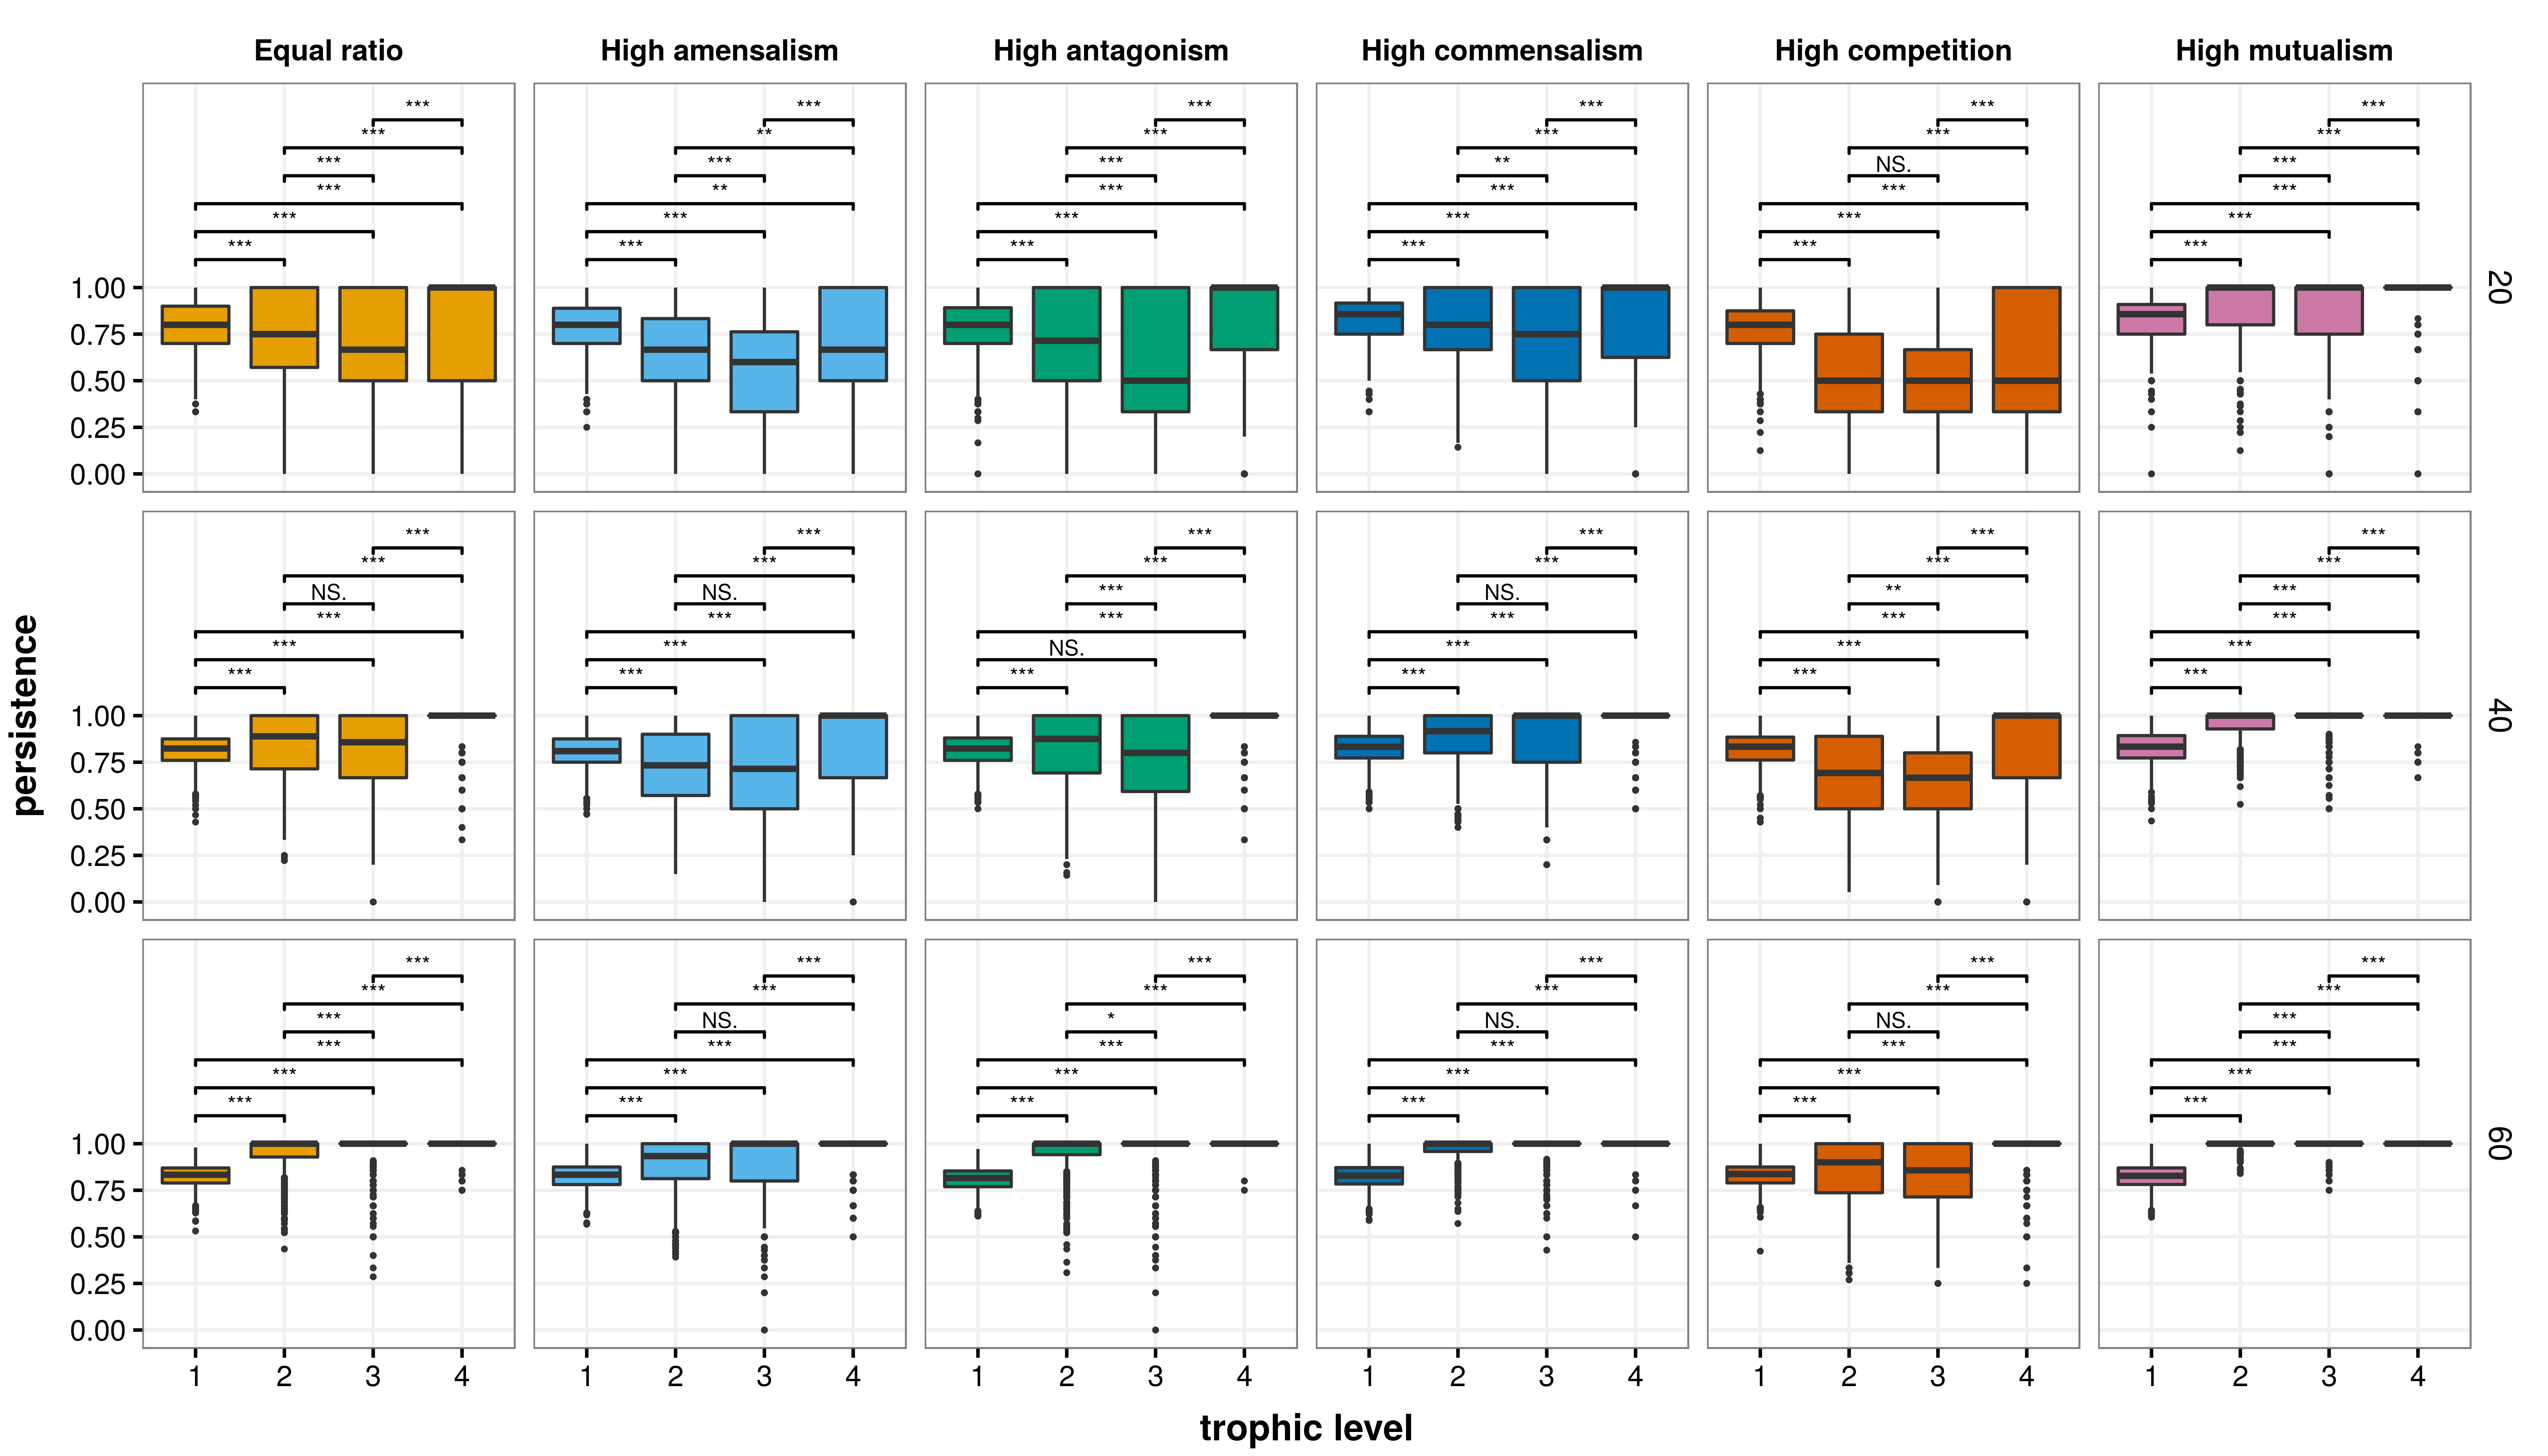
\includegraphics[width=\textwidth]{./Figures/Appendix3_2/Fig_1.png}
\caption[Persistence by trophic level]{\color{Gray} Persistence values of the main simulations grouped by initial richness, interaction frequencies, and trophic level. The line inside the boxes represents the median values, lower and upper hinges correspond to the first and third quantiles and whiskers extend to the smallest/largest value no further than 1.5 times the inter-quartile range. Bars and symbols above the boxplots represent the outcome of Wilcoxon signed-rank tests (corrected for multiple comparisons with the Bonferroni correction) for the difference between pairs of groups (N.S: not significant, * p \textless{} 0.05, ** p \textless{} 0.01, *** p \textless{} 0.001).}
\label{fig:figApp3.2.1}
\end{figure}

\begin{figure}[!ht]
\centering
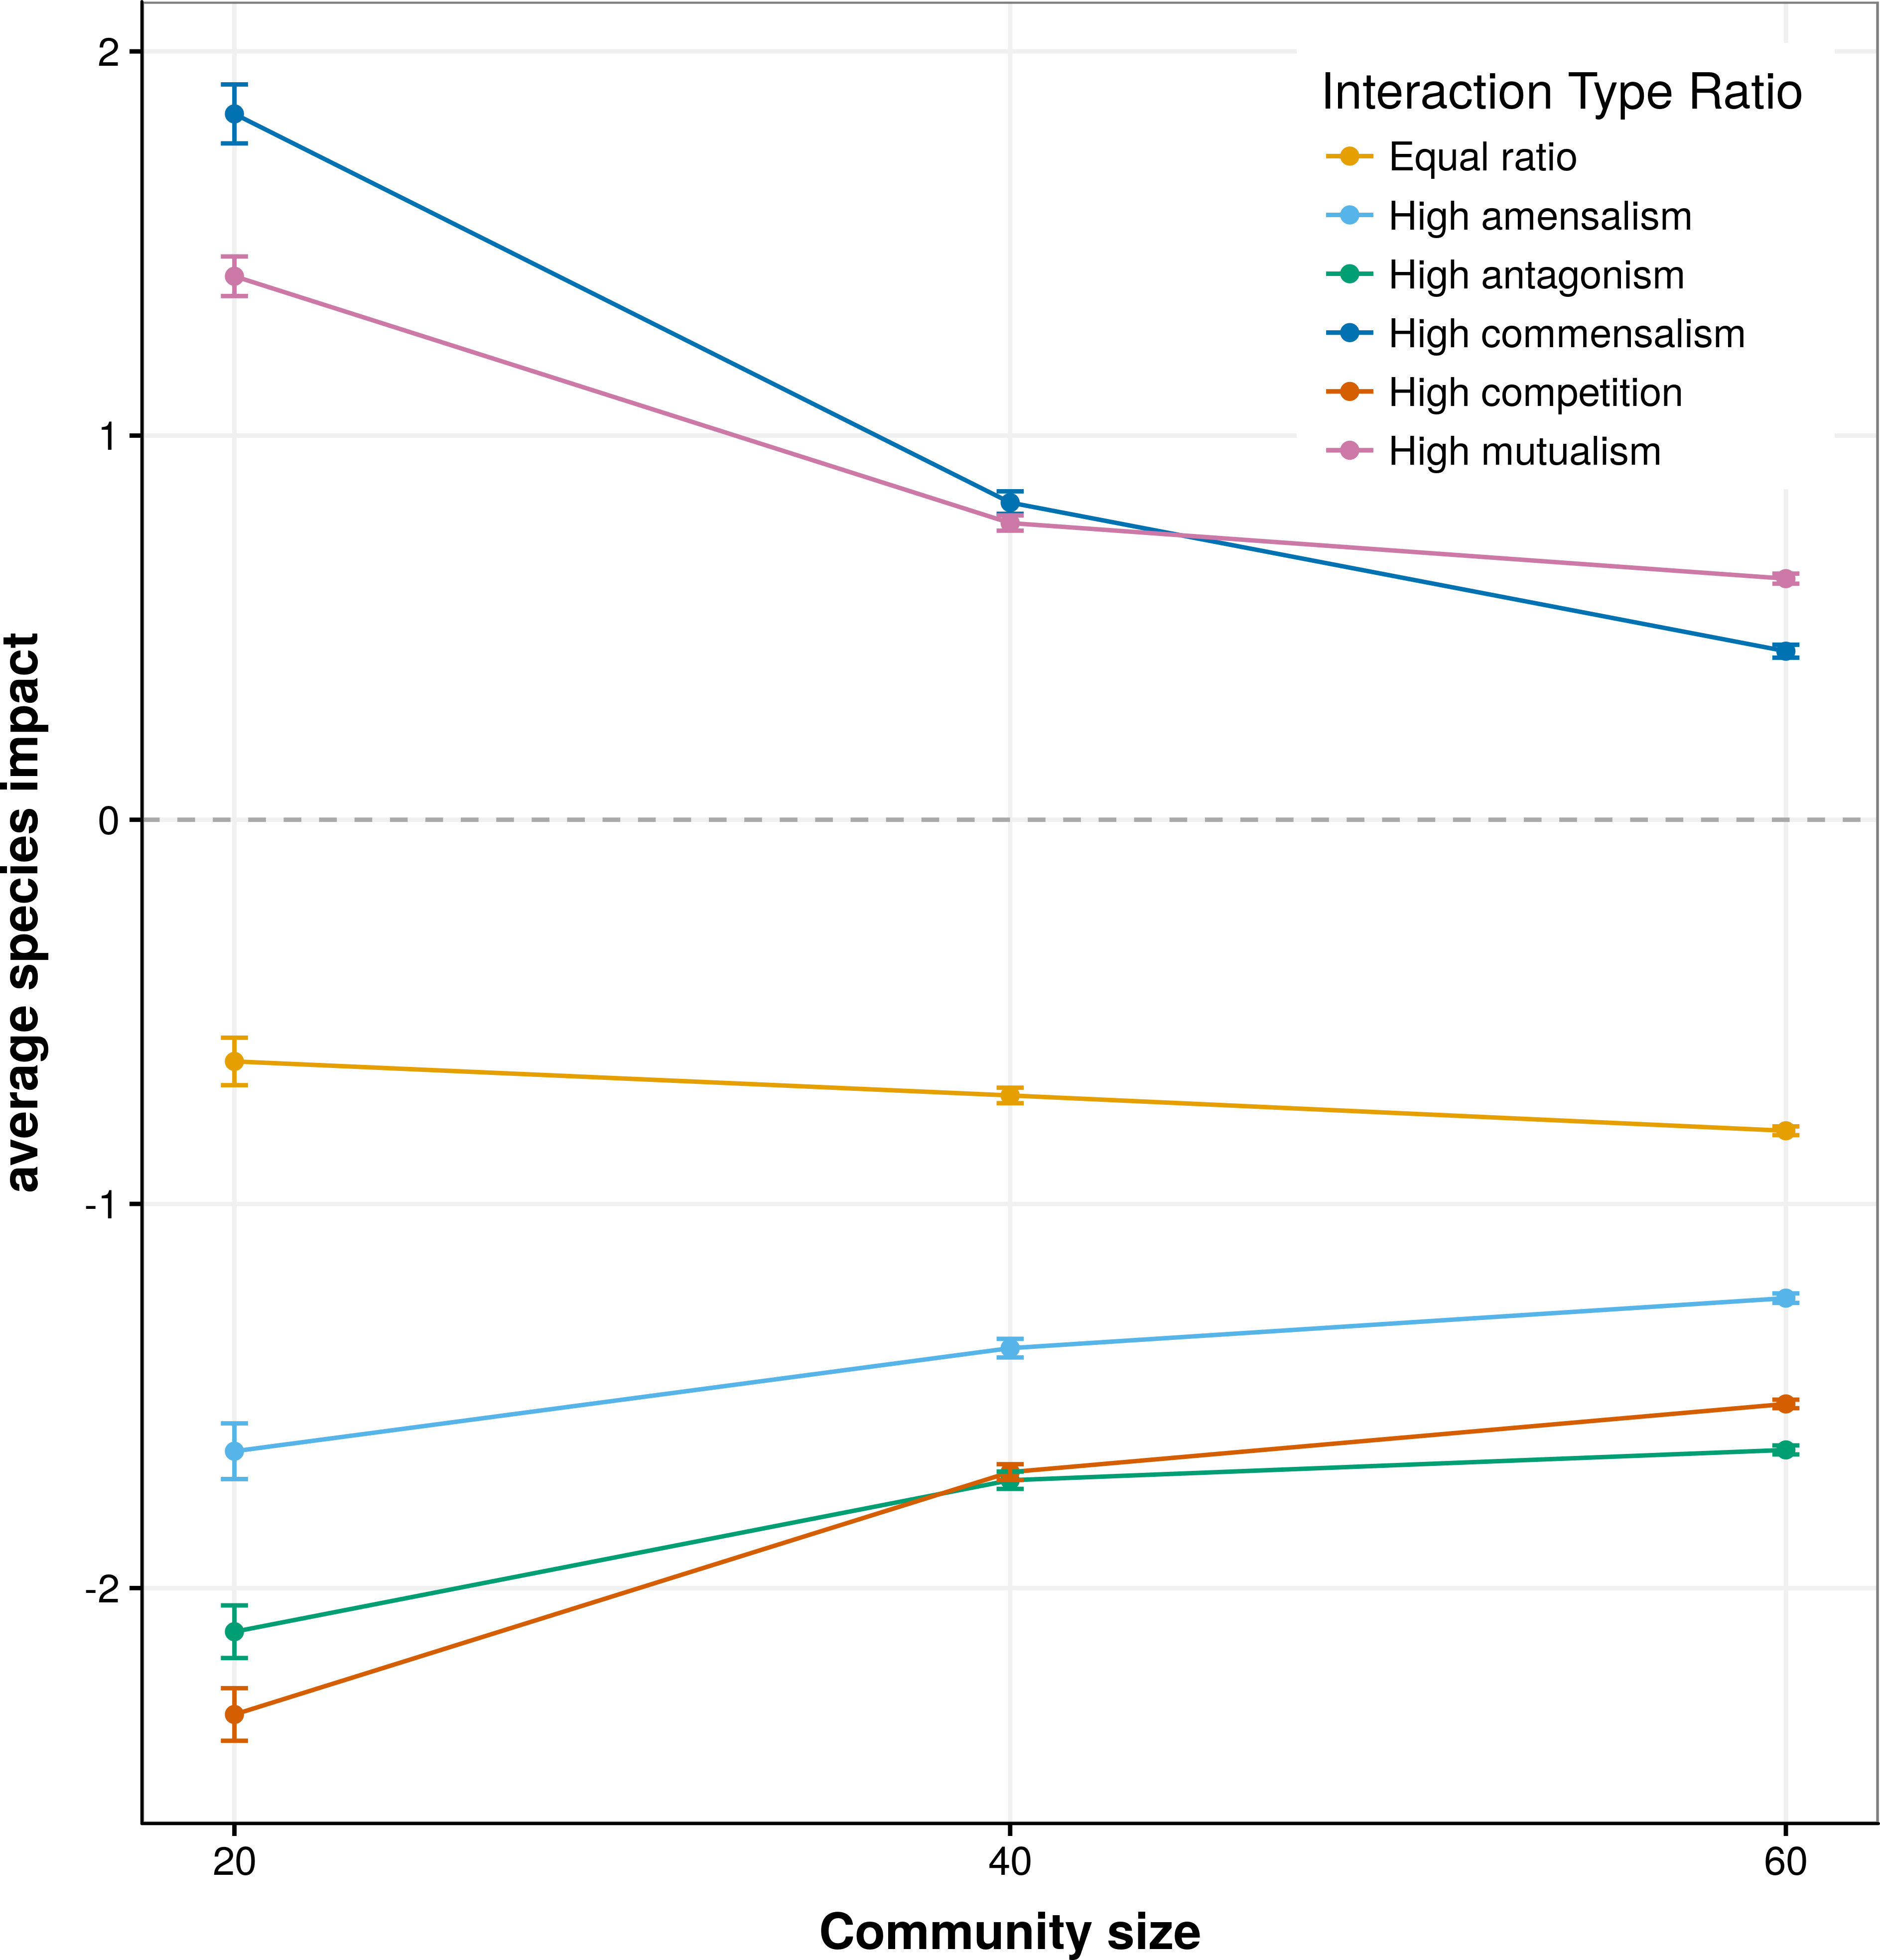
\includegraphics[width=.7\textwidth]{./Figures/Appendix3_2/Fig_2.png}
\caption[Impact by interaction frequency]{\color{Gray} Average pairwise species impact in model communities grouped by initial richness and interaction frequencies. Error bars represent standard error.}
\label{fig:figApp3.2.2}
\end{figure}
